\section{Flat plates or flat slabs }
Since early 1950s the trend toward lighter and more flexible construction configurations led to the rise of flat plates, particularly for medium- to high-rise office and residential buildings\citep{Fema2741997} although it was originally patented years earlier\citep{usp1899,hill1900,usp1909,usp1925} thoroughly reviewed in \cite{gasparini2002contributions}(\ref{t1905f6}). Due to their beamless nature and being free of obstructions, flat slabs provide many advantages such as lower story height, better lighting and ventilation, arrangement of piping and wiring, more clear space in addition to architectural flexibility and easier formwork in construction. 

\begin{figure}\centering
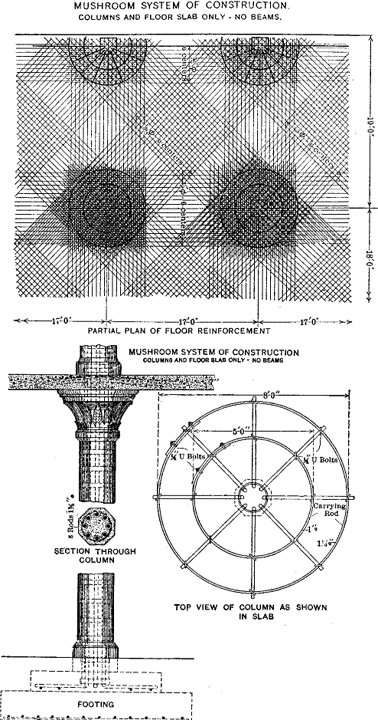
\includegraphics[width=\columnwidth]{Figures/t1905f6.png}
\caption{Turner's ``Mushroom'' flat-slab concept\citep{turner1905}.}\label{t1905f6}
\end{figure}

Despite the architectural charm this system doesn't have a well established seismic reputation and due to it's vulnerability to seismic loads it's behavior is normally a matter of concern\footnote{This doesn't make one wonder why \citet[Table 6.6.3.1.1]{aci31819} applies the lowest inertia moment factor ($0.25$) to flat slabs and flat plates for elastic analysis at factored load levels.}\citep{HosahalliSomaprasadR1994SVoF,Derecho2001}. Research on two-way flat slabs with drop panels indicates that in this particular case they have similar behavior to flat plates\citep{odello1967behavior}. It's notable that detailing requirements for two-way slabs without beams as mentioned earlier for flat plates in \citet[Chapter 21]{aci31895} appear only in the section relating to areas of moderated seismic risk which in turn suggests that \cite{aci31895} considers the use of flat plates as acceptable components of the lateral-load-resisting system only for areas of moderate seismicity\citep{Derecho2001}. Punching shear failure at slab-column connection for this system because of its brittle nature and potential in triggering progressive collapse may lead to catastrophic losses as evidenced in the collapses of the 2000 Commonwealth Avenue building\citep{king2004} and the Sampoong department store building\citep{PARK2012119}.
    
Ductile detailing of all structural connections, including also for those with only gravity load has become a key concept that was learned as a result of failures observed during the 1971 San Fernando Valley Earthquake. Slab-column connections in a flat plate structure though only gravity loaded must maintain load bearing capacity at maximum lateral displacement allowed by the lateral load bearing system during which there is chance of brittle failure modes like slab punching shear taking place if this displacement is not absorbed by slab-column interfaces\citep{DoD2016}. This mode of failure could occur with little or no warning signs that has resulted in the progressive collapse of this type of structures as in the 1985 Mexico City earthquake in which 91 flat plate buildings collapsed and 44 others were severely damaged due to punching failure\citep{ghali2000stud}. Unfortunately flat slab performance remained poor in the 2017 Mexico City earthquake also\citep{isufi2020}. Although punching failure occurs during the earlier stages of construction too, when concrete has yet to harness reliable strength to resist shear effects\citep{gardner2011}. 

The Iranian code of standard practice for seismic design of buildings\citep[Section 3-3-5-5]{28002014} restricts the use of flat slabs either with or without drop panels to buildings at maximum 3 stories or 10m tall. Whereas in \cite{aci31819} slab-column frames without beams are at most accounted as intermediate moment frames and per \citet[Section R18.2]{aci31819} are not permitted as part of seismic-force-resisting systems for structures assigned to Seismic design classification (SDC) D, E, or F and are only allowed as a gravity or secondary system where shear walls form the seismic or lateral force resisting system (SFRS or LFRS). The reasoning for this simply put by \citet[Chapter 7]{JointACI-ASCECommittee4212015} is that these frames cannot meet the detail requirements for the level of energy dissipation and ductility demanded for special moment frames. Even when an independent lateral-force-resisting system is provided \cite{JointACI-ASCECommittee4212015} suggests that flat plate-column connections should be designed to accommodate the moments and shear forces associated with the displacements or story drifts during earthquakes. Thus all members in slab-column frames not designated as part of the SFRS should be designed to support gravity loads while subjected to design displacements.  

During the recent decades various laboratory tests concerning flat slabs have been carried out which are distinguishable in three specimen size classes as \begin{itemize}\item isolated slab-connections, \item complete single floors, \item and complete frames at least two stories tall. \end{itemize}
Numerous research has dominated the field as presented herein studying isolated slab-column connections under combined gravity and lateral loading\citep{dovich2005,drakatos2016,hawkins1979,hueste2007,kang2006,megally2000,pan1989,robertson2002,setiawan2019,tian2008,andre2016} while fewer have been in the form of size scaled floors tested under cyclic loads\citep{hwang1993,hwang2000,rha2014} and only four consisted of complete buildings\citep{coronelli2021,fick2017,moehle1984,kang2004}. \cite{coronelli2020} provides an state of the art review of these larger scale tests and an introduction to the ``Slab STRESS'' research program reported by \cite{coronelli2021} in which a full-scale flat slab specimen is tested. \cite{coronelli2021} carried out seismic tests for service and ultimate actions using pseudodynamic technique with virtual walls in which the flat slab frame was the secondary element as suggested by \cite{asce4117,fema356}\footnote{\cite{asce4117} classifies building components as either primary or secondary in respect to their role in resisting the seismic forces and whether their failure or degradation would compromise building lateral stability, thus secondary elements would be any building structural element whose purpose is to support gravity loads. \cite{asce4117} requires that both primary and secondary components be evaluated to confirm their seismic force and deformations do not behave inconsistently with the selected performance level therefore the standard also states that where a component intended in the original building design as primary is deformed beyond the point where it can be relied to resist earthquake effects, the secondary designation may be used.}. \cite{chen2023} experimentally investigated the effects of spatial steel drop panel plate components on punching shear performance of slab-column connections with five interior slab-column subassemblages tested under gravity load.

Moment and crack distribution and redistribution in multi bay slab column frames due to nonlinear behavior and progressive deterioration of joints are major draw backs for isolated connection subassemblies which might fail at providing accurate boundary conditions\citep{einpaul2015,einpaul2016}. \cite{einpaul2015} investigated moment redistribution between hogging and sagging moments and compressive membrane action influence on conventional isolated connection experiments suggesting that the punching capacity of continuous slabs with low amounts of flexural reinforcement on the interior column regions may be underestimated in the codes of practice. Note that there are plenty of tests on internal slab-column connection specimens while results for edge or corner columns are less frequent. 

